\section{Clinical-evidence audit: the panel is indication-diffuse (CIViC)}
The gnomAD and GTEx audits rule out germline and expression-level sources of
pancreatic specificity for the four detection-panel genes. Here we ask the same
question of the \emph{curated clinical-evidence base} itself, using the CIViC
v2 knowledgebase (\texttt{civicdb.org} GraphQL API): every evidence item whose
molecular-profile name mentions each gene was retrieved (all curation statuses;
accepted items analyzed), one row per unique evidence identifier (EID), giving
1,146 unique EIDs across the six genes audited
(\texttt{results/civic\_panel\_evidence\_rows.csv}).

Two positive controls calibrate the metric. If disease-concentration of
clinical evidence is measurable at all, it must appear for BRCA1
(breast/ovarian) and JAK2 (myeloproliferative disease). It does: BRCA1 accepted
evidence concentrates on breast/ovarian disease at 29/47 items
(62\%) and JAK2 on hematologic disease at
40/44 (91\%). Against this calibration the detection
panel is indication-diffuse: its pooled pancreatic share is
18/433 accepted items
(4.2\%, 95\% CI 2.6--6.5\%), far below either control
(Fisher $p=3.7e-22$ and $p=1.6e-39$).

\begin{table}[h]\centering\footnotesize
\begin{tabular}{@{}lrrrp{4.9cm}@{}}
\hline
Gene & accepted & pancreatic & share & top accepted diseases \\ \hline
KRAS & 200 & 13/200 & 6.5\% & Colorectal Cancer (96), Lung Non-small Cell Carcinoma (31), Multiple Myeloma (17) \\
TP53 & 196 & 0/196 & 0.0\% & Cancer (21), Breast Cancer (16) \\
CDKN2A & 30 & 2/30 & 6.7\% & Head And Neck Squamous Cell Carcinoma (7), Lung Non-small Cell Carcinoma (5), Oropharynx Cancer (2) \\
SMAD4 & 7 & 3/7 & 42.9\% & Colorectal Cancer (2), Pancreatic Adenocarcinoma (1), Pancreatic Ductal Adenocarcinoma (1) \\ \\ \hline
\end{tabular}
\caption{CIViC accepted evidence items per panel gene. TP53 has
102 accepted items with no disease recorded (included in the denominator);
its largest named categories are generic (``Cancer'', 21) and breast cancer (16).}
\end{table}

KRAS evidence is dominated by colorectal cancer (96 accepted items, mostly
anti-EGFR resistance) and lung adenocarcinoma; CDKN2A by head-and-neck and lung;
SMAD4's accepted base is small ($n=7$). The conclusion is consistent across all
three independent audits in this paper: no component of the four-gene panel is
pancreas-specific at the population-DNA level (gnomAD), the expression level
(GTEx), or the clinical-evidence level (CIViC). Pancreatic specificity of a
cfDNA assay on this panel must therefore come from the \emph{mutation-pattern
combination} (the CNN/GNN score over the joint panel), not from any single
marker.

\begin{figure}[h]\centering
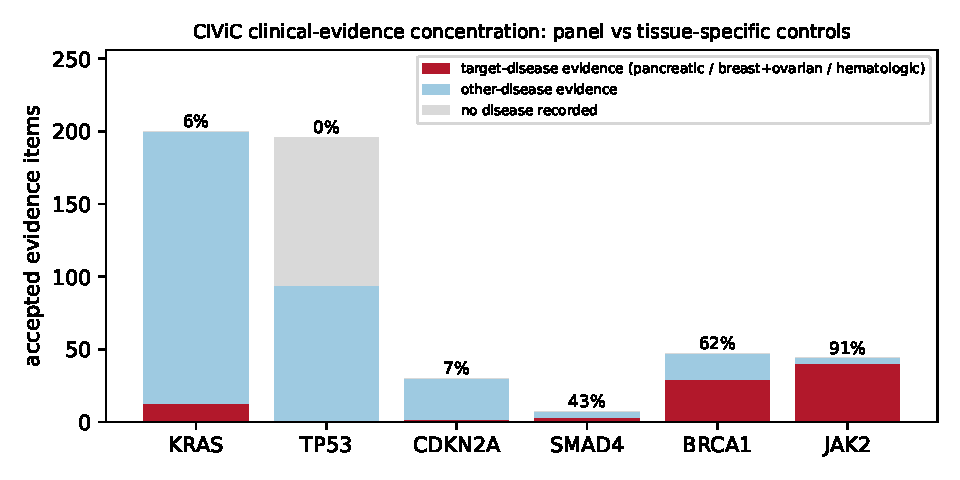
\includegraphics[width=0.82\linewidth]{figs/fig_civic.pdf}
\caption{Accepted CIViC evidence items per gene, split into target-disease
evidence (red: pancreatic for the panel, breast+ovarian for BRCA1, hematologic
for JAK2), other-disease evidence (blue), and items with no disease recorded
(grey). Percentages above bars give the target-disease share.}
\label{fig:civic}\end{figure}
